\begin{frame}[c]{Le motivazioni alla base di questo lavoro}

placeholder

\vspace{0.5cm}
placeholder

\end{frame}

\begin{frame}[c]{Roadmap}

\begin{itemize}
\item Il progetto SeismoCloud
\item Architettura del sistema SeismoCloud EUD
\item Implementazione delle funzionalità
\item Sicurezza e protezione dei dati
\item Test
\item Sviluppi futuri
\end{itemize}

\end{frame}

\section{Il progetto SeismoCloud}

\section{Architettura del sistema SeismoCloud EUD}

\section{Implementazione delle funzionalità}

\section{Sicurezza e protezione dei dati}

\section{Test}

\section{Sviluppi futuri}

\begin{frame}[c]{Sviluppi futuri}

\begin{enumerate}
	\item Integrazione di funzionalità per \textit{Social Network} e \textit{Smart home}
	\item Ottimizzazione delle prestazioni tramite la condivisione di un solo client MQTT
	\item Metodo di accesso sicuro ed affidabile a SeismoCloud Node-RED
\end{enumerate}

\end{frame}

\begin{frame}
\begin{figure}
    \centering
    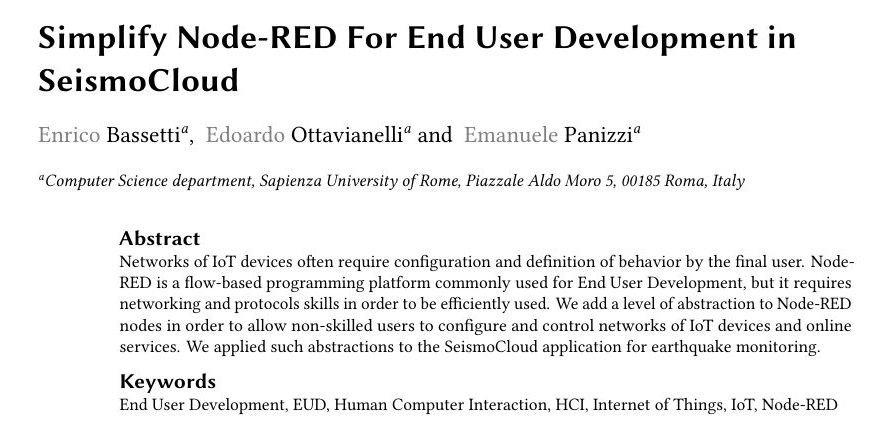
\includegraphics[width=1\textwidth]{images/paper.jpg}
    \label{fig:paper}
\end{figure}
\end{frame}

\revslide{Grazie}
